% !TEX program = xelatex
\documentclass[UTF8,11pt,a4paper,fontset=fandol]{ctexart}

\usepackage[a4paper,margin=2.35cm,headheight=15pt]{geometry}
\usepackage{amsmath,amssymb}
\usepackage{booktabs,tabularx,array,multirow}
\usepackage{enumitem}
\usepackage{xcolor}
\usepackage{tikz}
\usepackage{hyperref}
\usepackage{fancyhdr}
\usepackage{microtype}
\usepackage{tcolorbox}
\usepackage{listings}
\usepackage{caption}
\usepackage{float}

\usetikzlibrary{arrows.meta,positioning,fit,calc,backgrounds}

\definecolor{RPBlue}{HTML}{2456A6}
\definecolor{RPCyan}{HTML}{168AAD}
\definecolor{RPGreen}{HTML}{2F855A}
\definecolor{RPOrange}{HTML}{C56A18}
\definecolor{RPRed}{HTML}{B33A3A}
\definecolor{RPGray}{HTML}{56616F}
\definecolor{RPLight}{HTML}{F3F6FA}
\definecolor{RPLine}{HTML}{D8E0EA}

\hypersetup{
  colorlinks=true,
  linkcolor=RPBlue,
  urlcolor=RPCyan,
  citecolor=RPGreen,
  pdftitle={Research-Pi：面向计算实验科研的 Project-Centric Agent Harness},
  pdfauthor={Research-Pi 项目}
}

\pagestyle{fancy}
\fancyhf{}
\lhead{Research-Pi 设计思想与阶段成果}
\rhead{\thepage}
\renewcommand{\headrulewidth}{0.4pt}

\setlist[itemize]{leftmargin=2em,itemsep=0.25em,topsep=0.35em}
\setlist[enumerate]{leftmargin=2em,itemsep=0.25em,topsep=0.35em}
\renewcommand{\arraystretch}{1.22}
\setlength{\parindent}{2em}
\setlength{\parskip}{0.25em}

\newcolumntype{Y}{>{\raggedright\arraybackslash}X}
\newcommand{\code}[1]{\texttt{#1}}
\newcommand{\term}[1]{\textbf{#1}}
\newcommand{\memtag}[1]{\fcolorbox{RPGreen}{RPGreen!8}{\strut\footnotesize\bfseries #1}}

\newtcolorbox{resultbox}[1][]{
  colback=RPLight,
  colframe=RPBlue,
  boxrule=0.8pt,
  arc=2pt,
  left=8pt,right=8pt,top=7pt,bottom=7pt,
  title=#1,
  fonttitle=\bfseries
}

\lstset{
  basicstyle=\ttfamily\small,
  backgroundcolor=\color{RPLight},
  frame=single,
  rulecolor=\color{RPLine},
  breaklines=true,
  columns=fullflexible,
  showstringspaces=false
}

\title{\bfseries Research-Pi：面向计算实验科研的\\Project-Centric Agent Harness\\\large 设计思想、系统实现与阶段成果汇报}
\author{Research-Pi 项目}
\date{\today}

\begin{document}

\maketitle

\begin{resultbox}[结论先行]
Research-Pi 不是 AutoResearch，也不只是给 Coding Agent 增加科研提示词。它面向研究者深度参与的计算实验流程，用三条轴组织 Harness：\term{记忆 $M$}让 Session 可以丢弃而研究认知留下，\term{通信 $C$}让 User、Leader 与 Subagent 的任务和消息不串扰，\term{控制 $A$}让 Agent 在项目内充分执行而人的研究裁决不可替代。当前工程机制已经通过自动化测试和真实项目迭代；是否提高科研效率与结论质量，仍需在后续科研任务中评估。
\end{resultbox}

\setcounter{tocdepth}{2}
\tableofcontents
\newpage

\section{模块一：动机与目标}

\subsection{为什么通用 Coding Agent 不足以承担长程科研}

计算实验科研并不只是连续写代码。研究者需要反复提出假设、设计可区分实验、检查结果是否有效，并据此改变方向。通用 Coding Agent 在这一过程中主要暴露三类问题：

\begin{enumerate}
  \item \term{目标错位}：倾向最小改动、完成当前任务和保护已有实现，而科研早期更需要高信息增益实验、快速证伪和果断放弃弱路线。
  \item \term{上下文污染}：计划、命令、日志和中间补丁不断进入同一 Session，真正的研究问题与证据边界逐渐被工具噪声淹没。
  \item \term{模型固有惯性}：GPT 类模型容易沿最近任务继续局部修补，把流畅解释当成可靠结论，把进程 \code{completed}、任务完成和假设成立混为一谈；长上下文与有损摘要还会放大旧判断的惯性。
\end{enumerate}

因此，Research-Pi 不是要构造无人参与的 AutoResearch，而是要构造一个\term{研究者能够深度参与的 Research Harness}：Agent 承担记忆恢复、候选假设、工具执行和证据整理；人持续提供研究目标、价值判断、关键取舍和对结论的最终裁决。人的作用不是异常时才介入的审批器，而是研究闭环中不可替代的共同决策者。

\section{模块二：三轴设计}

\subsection{一张图理解 Research-Pi}

Research-Pi 将 Harness 归纳为三个相互耦合的轴：记忆 $M$ 维持跨时间的研究连续性，通信 $C$ 维持跨 Actor 的任务连续性，控制 $A$ 决定谁可以把判断变成现实行动。

\begin{figure}[H]
  \centering
  \begin{tikzpicture}[
    node distance=12mm and 17mm,
    box/.style={draw=RPLine, very thick, rounded corners=2pt, minimum height=12mm, text width=2.55cm, align=center, fill=white, inner sep=5pt, font=\small},
    human/.style={box, draw=RPBlue, fill=RPBlue!7},
    agent/.style={box, draw=RPCyan, fill=RPCyan!7},
    memory/.style={box, draw=RPGreen, fill=RPGreen!8},
    control/.style={box, draw=RPOrange, fill=RPOrange!9},
    arrow/.style={-{Latex[length=2.3mm]}, thick, draw=RPGray},
    flow/.style={{Latex[length=2.3mm]}-{Latex[length=2.3mm]}, thick, draw=RPGray}
  ]
    \node[human] (user) {User\\目标与最终裁决};
    \node[agent, right=of user] (leader) {Pi Leader\\规划与解释};
    \node[agent, right=of leader] (sub) {Subagent\\Advisor / Executor};
    \node[memory, below=of user] (mem) {Memory $M$\\证据、状态、ProjectView};
    \node[control, below=of leader] (auth) {Control $A$\\角色、权限、恢复};
    \node[box, below=of sub] (work) {Actions\\代码、实验、SSH};

    \node[font=\small\bfseries, text=RPCyan] at ($(user.north)!0.5!(sub.north)+(0,7mm)$) {Communication $C$};
    \draw[flow] (user) -- (leader);
    \draw[flow] (leader) -- (sub);
    \draw[arrow] (mem) -- (leader);
    \draw[arrow] (leader) -- (auth);
    \draw[arrow] (sub) -- (work);
    \draw[arrow] (auth) -- (work);
    \draw[arrow] (work.south) |- (mem.south);
  \end{tikzpicture}
  \caption{Research-Pi 的三轴闭环。上层通信 $C$ 连接 User、Leader 与 Subagent；控制 $A$ 约束它们能够触发的现实行动；行动产生的证据回到记忆 $M$，再通过 ProjectView 和检索进入下一轮判断。}
  \label{fig:three-axes}
\end{figure}

\begin{table}[H]
  \centering
  \caption{三轴分别解决什么问题}
  \small
  \begin{tabularx}{\textwidth}{>{\bfseries\raggedright\arraybackslash}p{1.7cm}p{4.1cm}Y}
    \toprule
    轴 & 核心问题 & 在 Research-Pi 中的体现 \\
    \midrule
    记忆 $M$ & 哪些历史可信、当前研究状态是什么、本轮模型需要看到什么 & 原始 Session/Artifact、实验账本、全文检索、structured compact、ProjectView \\
    通信 $C$ & 谁在处理哪个目标，问题、进度和结果应送给谁 & User--Leader 对话、Actor/Action、mission/thread、durable mailbox、ASK/result、Session handoff \\
    控制 $A$ & 谁能读写或执行，哪些决策必须由人裁决，副作用未知时如何恢复 & Leader/Analysis 角色、project sandbox、host capability、SSH trust、preflight、cancel/reconcile \\
    \bottomrule
  \end{tabularx}
\end{table}

\subsection{M：四类扩展把历史变成模型可用的研究状态}

“原始、结构化、工作”描述的是记忆层级，不是扩展名称。Research-Pi 中真正对应的四类功能如下：

\begin{table}[H]
  \centering
  \caption{记忆扩展的职责与层级}
  \small
  \setlength{\tabcolsep}{4pt}
  \begin{tabularx}{\textwidth}{>{\raggedright\arraybackslash}p{3.8cm}YY}
    \toprule
    扩展功能 & 它具体做什么 & 在记忆层级中的作用 \\
    \midrule
    \memtag{M1}\quad\term{原始检索}\par\smallskip
    \term{Research Memory}\par{\footnotesize Search / Read}
    & 为完整 Session JSONL、实验记录和历史条目建立本地全文索引；先返回 session/entry 引用，再读取小范围原文
    & \term{原始历史的检索入口}。原文保留最高信息量，但不会自动进入每轮上下文 \\
    \addlinespace[2pt]\cmidrule(lr){1-3}\addlinespace[2pt]
    \memtag{M2}\quad\term{证据账本}\par\smallskip
    \term{Experiment Ledger}
    & \code{record\_experiment} 保存 intervention、observation、validity、interpretation 与 provenance；transition 保存研究换轨
    & \term{结构化证据记忆}。记录“发生了什么及是否可解释”，但不自动代表当前结论 \\
    \addlinespace[2pt]\cmidrule(lr){1-3}\addlinespace[2pt]
    \memtag{M3}\quad\term{长期状态}\par\smallskip
    \term{Project State}
    & Research Compact 在阶段检查点综合 research question、claim、竞争假设、观察、决策、混淆因素和下一实验；状态按 revision 持久化，也可通过 amendment 做小范围修订
    & \term{Project 级持久状态}。回答“当前依据什么相信什么”，跨 Session 共享且带 provenance \\
    \addlinespace[2pt]\cmidrule(lr){1-3}\addlinespace[2pt]
    \memtag{M4}\quad\term{调用视图}\par\smallskip
    \term{ProjectView}
    & 从 Project State、最新 evidence/transition、task handoff、Git 与 Runtime 状态确定性地渲染限长视图；按需要发送完整 snapshot 或短 delta
    & \term{模型可见的项目视图}。回答“这次调用需要看到什么”，带 freshness，但不形成新的研究状态 \\
    \bottomrule
  \end{tabularx}
\end{table}

\newpage
四层并不互相替代：Research Memory 找回精确来源，Experiment Ledger 保存证据，Research Compact 在阶段检查点形成 Project State，ProjectView 再把 Project State 与其后发生的新变化投影到 Model Context。\term{M3 是持久状态，M4 是调用视图}：snapshot 与 delta 只是 ProjectView 的完整和增量传递形式，不是另一份状态。新 evidence 可以先出现在 ProjectView 中，但在 compact 或 amendment 前仍标记为“尚未综合”，不能反向覆盖 Project State。

\noindent\textit{形成与投影：Research Compact 是形成过程，Project State 是持久结果，ProjectView 是面向模型的投影。Compact Summary 与完整 ProjectView 会共享部分核心字段；前者维持 Session 连续性，后者负责跨 Session 定向和最新状态校正。}

\subsection{C：消息沿 Project Runtime 路由，而不是绑定某个聊天窗口}

\begin{figure}[H]
  \centering
  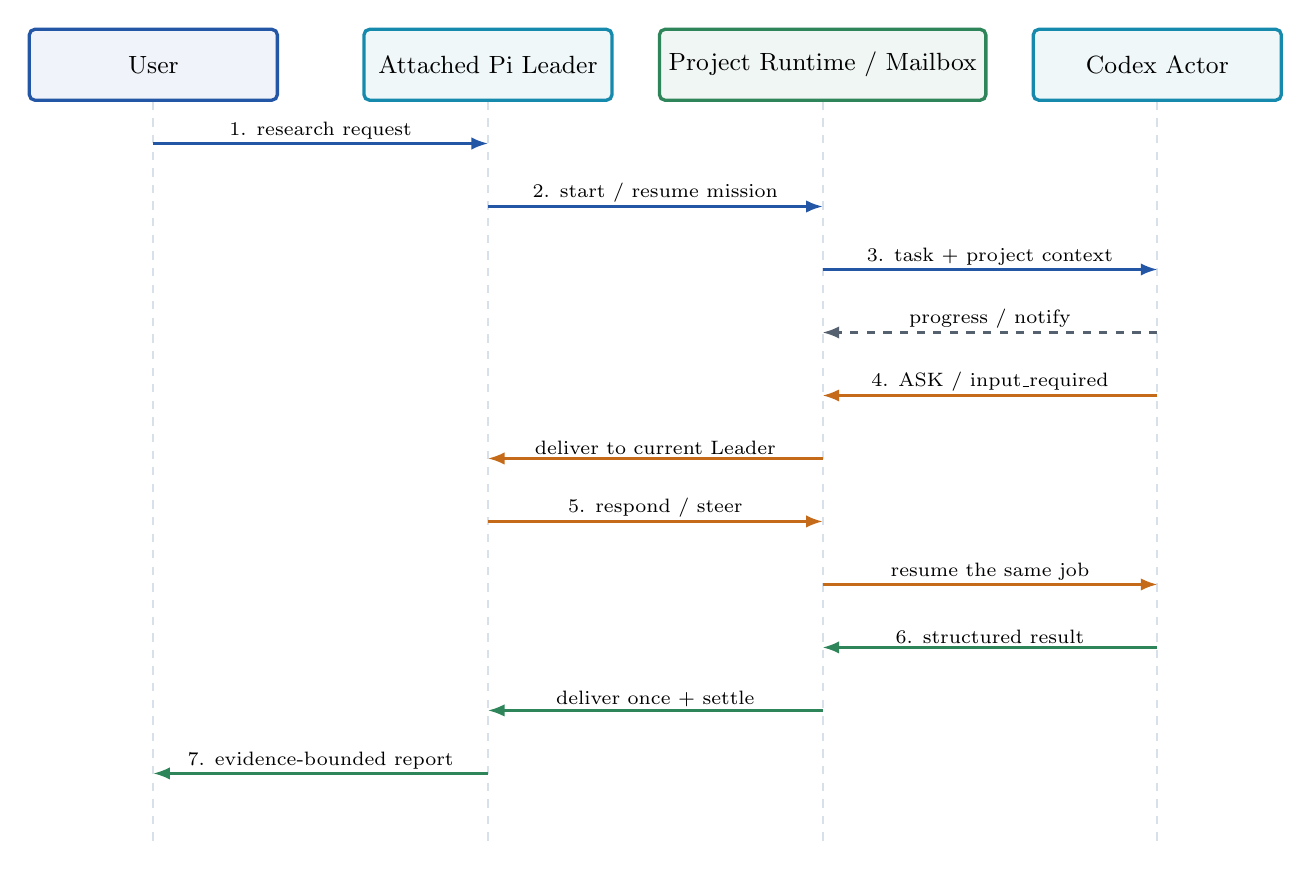
\begin{tikzpicture}[
    x=1cm,y=1cm,
    actor/.style={draw=RPCyan, very thick, rounded corners=2pt, minimum width=3.15cm, minimum height=9mm, align=center, fill=RPCyan!7, font=\small},
    human/.style={actor, draw=RPBlue, fill=RPBlue!7},
    runtime/.style={actor, draw=RPGreen, fill=RPGreen!7},
    life/.style={draw=RPLine, dashed, thick},
    msg/.style={-{Latex[length=2.1mm]}, thick},
    taskmsg/.style={msg, draw=RPBlue},
    askmsg/.style={msg, draw=RPOrange},
    resultmsg/.style={msg, draw=RPGreen},
    async/.style={msg, draw=RPGray, dashed}
  ]
    \node[human] (u) at (0,0) {User};
    \node[actor] (l) at (4.25,0) {Attached Pi Leader};
    \node[runtime] (r) at (8.5,0) {Project Runtime / Mailbox};
    \node[actor] (c) at (12.75,0) {Codex Actor};

    \foreach \n in {u,l,r,c}{\draw[life] (\n.south) -- ++(0,-9.4);}

    \draw[taskmsg] (0,-1.0) -- node[above,fill=white,inner sep=1pt,font=\scriptsize]{1. research request} (4.25,-1.0);
    \draw[taskmsg] (4.25,-1.8) -- node[above,fill=white,inner sep=1pt,font=\scriptsize]{2. start / resume mission} (8.5,-1.8);
    \draw[taskmsg] (8.5,-2.6) -- node[above,fill=white,inner sep=1pt,font=\scriptsize]{3. task + project context} (12.75,-2.6);
    \draw[async] (12.75,-3.4) -- node[above,fill=white,inner sep=1pt,font=\scriptsize]{progress / notify} (8.5,-3.4);
    \draw[askmsg] (12.75,-4.2) -- node[above,fill=white,inner sep=1pt,font=\scriptsize]{4. ASK / input\_required} (8.5,-4.2);
    \draw[askmsg] (8.5,-5.0) -- node[above,fill=white,inner sep=1pt,font=\scriptsize]{deliver to current Leader} (4.25,-5.0);
    \draw[askmsg] (4.25,-5.8) -- node[above,fill=white,inner sep=1pt,font=\scriptsize]{5. respond / steer} (8.5,-5.8);
    \draw[askmsg] (8.5,-6.6) -- node[above,fill=white,inner sep=1pt,font=\scriptsize]{resume the same job} (12.75,-6.6);
    \draw[resultmsg] (12.75,-7.4) -- node[above,fill=white,inner sep=1pt,font=\scriptsize]{6. structured result} (8.5,-7.4);
    \draw[resultmsg] (8.5,-8.2) -- node[above,fill=white,inner sep=1pt,font=\scriptsize]{deliver once + settle} (4.25,-8.2);
    \draw[resultmsg] (4.25,-9.0) -- node[above,fill=white,inner sep=1pt,font=\scriptsize]{7. evidence-bounded report} (0,-9.0);
  \end{tikzpicture}
  \caption{Codex 消息先进入 Project Runtime，再交给当前 attached Leader。蓝色 1--3 是任务路径，橙色 4--5 是阻塞 ASK 往返，绿色 6--7 是结果路径；灰色虚线 progress 只供 \code{/watch} 观察。ASK 通过精确的 job ID 和 request ID 返回同一 Codex turn；Session 轮换只改变 Leader attachment，不改变 Action、mailbox 和 mission 的 Project 归属。}
  \label{fig:communication-sequence}
\end{figure}

\par\medskip
\noindent\term{三条关键消息路径如下：}

\begin{itemize}
  \item \term{任务路径}：Leader 用稳定 mission 启动或续接 Action；Runtime 绑定 Project、workspace、mode、research track 和 Codex thread，防止另一个 Session 或分支误接任务。
  \item \term{阻塞路径}：Codex 需要信息或权限时发送 ASK/\code{input\_required}。mailbox 将它交给当前 Leader；\code{respond} 回答明确请求，\code{steer} 在安全边界修正方向，二者都续接原 job，而不是重启一个新 Agent。
  \item \term{结果路径}：progress/notify 主要进入状态栏和 \code{/watch}；terminal result 只投递一次并保留结构化 outcome、changed files、checks、external effects 与 remaining work。Leader 进行有效性判断后再向 User 汇报或写入证据记忆。
\end{itemize}

Mailbox 消息经历 \code{queued → delivered → consumed/superseded}，因此“模型看见 ASK”不等于请求已经结算，旧 ASK 也不会永久复活。Analysis Session 的 synthesis 通过同一 Runtime 作为 proposal 发给 Leader，但它不能消费 Leader mailbox 或直接更新 Project State。通信轴由此维持任务连续性，同时保持 Session 隔离。
\subsection{A：让 Agent 放手执行，让人保留研究裁决}

控制轴不是为了把 Agent 变成“乌龟”，而是把不同主体的权力说清楚：

\begin{itemize}
  \item \term{User}决定研究目标、关键取舍、项目外授权以及高代价或不可逆裁决；
  \item \term{Leader}在项目内规划、修改、运行实验和调度 subagent，并负责解释证据；
  \item \term{Subagent}在委派范围内咨询或执行；executor 可拥有与 Leader 相当的项目内权限，但不能取代 User/Leader 定义研究问题和更新结论；
  \item \term{Analysis Session}共享 Project memory，但保持只读；有价值的讨论作为 proposal 发给 Leader，只有用户显式 promote 后才获得执行权。
\end{itemize}

模型默认可在当前项目内读写、commit 和运行实验；项目外文件、精确 SSH target 与宿主命令通过 capability 明示越界，凭据本身不进入上下文。若 worker 中断且副作用未知，系统先检查 Git/run/远程状态并 reconcile，而不是盲目重跑。其好处是同时获得项目内执行自由、人的最终控制和可恢复的自动化。

\section{模块三：关键细节与当前证据}

\subsection{科研策略：先获得可靠信息，再做工程化}

Research Contract 把代码视为检验假设的工具：原因不明时形成实质不同的竞争假设，优先选择能区分它们的实验；负结果先检查介入是否生效；连续局部补丁没有增加信息量时主动换抽象或回到干净状态。只有方向获得证据支持后，才提高测试、兼容性与工程质量。该策略横跨三轴，但不另建一份 Project 状态。

\subsection{上下文与缓存：稳定前缀，动态尾部}

ProjectView 使用 append-only snapshot/delta：用户轮开始时把变化后的完整 snapshot 或短 delta 持久追加到 Session；同一轮工具刚产生的新 evidence、handoff 和 freshness 变化，只以临时 delta 放在当前请求尾部，下一用户轮再持久化。这样历史请求尽量保持为共同前缀，兼顾状态及时性与 DeepSeek KV-cache locality。Research compact 只在 agent 和工具链 settled 后触发；soft 阈值为 272K、hard 阈值为 384K，三档原始 recent tail 为 24K、32K 和 40K，加上目标约 8K 的结构化摘要后，compact 后通常约为 32K、40K 和 48K。缓存收益最终以 provider 的 cache-read tokens 判断，不由 Harness 自己宣布。

\subsection{一次模型调用：长前缀保持稳定，变化集中在尾部}

逻辑上，第 $t$ 个用户轮次中第 $k$ 次模型调用的完整请求可写为
\[
R_{t,k}=P\;\Vert\;H_{t-1}\;\Vert\;U_t\;\Vert\;W_{t,k}\;\Vert\;\Delta V_{t,k},
\]
其中 $P$ 是 Harness 前缀；$H_{t-1}$ 是持久 Session 历史，包含 compact summary、recent tail、既往消息以及已经持久化的 ProjectView snapshot/delta；$U_t$ 是当前用户请求；$W_{t,k}$ 是本轮已发生的 assistant/tool 消息；$\Delta V_{t,k}$ 是可选的尾部修正，只在同一轮中新 evidence 或 Runtime 变化尚未持久化时出现。$H$ 中的 ProjectView 消息与末尾 $\Delta V$ 属于同一个 ProjectView 机制，区别只是持久前缀与临时更新。

\begin{figure}[H]
  \centering
  \begin{tikzpicture}[
    x=1cm,y=1cm,
    layer/.style={draw=RPLine, very thick, rounded corners=2pt,
      minimum width=10.80cm, text width=10.15cm, align=left,
      inner xsep=8pt, inner ysep=5pt, font=\small},
    stable/.style={layer, fill=RPGreen!7, draw=RPGreen},
    turn/.style={layer, fill=RPBlue!6, draw=RPBlue},
    delta/.style={layer, fill=RPOrange!8, draw=RPOrange}
  ]
    \node[stable] (p) at (0,0) {%
      \term{P\quad Harness 固定前缀}\hfill
      \textcolor{RPGray}{来源：安装包与项目配置；更新：版本、模型或工具定义变化时}\\[-1pt]
      \footnotesize System prompt、Research Contract、项目规则、已加载 skills 与 tool schemas。它定义模型的角色、科研方法和可用动作。};

    \node[stable, below=2.5mm of p] (h) {%
      \term{$H_{t-1}$\quad 持久 Session 前缀}\hfill
      \textcolor{RPGray}{来源：上一轮已落定状态；更新：追加消息或 compact 时}\\[-1pt]
      \footnotesize Compact summary、保留的 recent tail、既往对话与工具结果，以及已经持久化的 ProjectView snapshot/短 delta 和已接收 mailbox。};

    \node[turn, below=5mm of h] (u) {%
      \term{$U_t$\quad 当前用户输入}\hfill
      \textcolor{RPGray}{来源：User；更新：每个用户轮次一次}\\[-1pt]
      \footnotesize 当前问题、约束、补充材料与显式授权。它给本轮推理确定目标，但不改写前面的历史证据。};

    \node[turn, below=2.5mm of u] (w) {%
      \term{$W_{t,k}$\quad 本轮增量轨迹}\hfill
      \textcolor{RPGray}{来源：Leader、工具与 Subagent；更新：本轮持续追加}\\[-1pt]
      \footnotesize assistant 推理外显、tool call/result、已接纳的 progress、ASK 与 RESULT。第 $k$ 次调用只在第 $k-1$ 次调用的尾部继续增长。};

    \node[delta, below=2.5mm of w] (d) {%
      \term{$\Delta V_{t,k}$\quad ProjectView 临时尾部修正}\hfill
      \textcolor{RPGray}{来源：语义状态变化；更新：必要时追加}\\[-1pt]
      \footnotesize 本轮刚产生、尚未持久化的 evidence、transition、handoff、Git/Runtime 与 mailbox freshness；无实质变化时不存在。};

    \draw[-{Latex[length=2.2mm]}, thick, draw=RPGray]
      ($(p.west)+(-7mm,3mm)$) -- node[left,align=right,font=\scriptsize,text=RPGray]
      {输入顺序\\从早到新} ($(d.west)+(-7mm,-3mm)$);

    \draw[very thick, draw=RPGreen]
      ($(p.east)+(5mm,3mm)$) -- ($(p.east)+(8mm,3mm)$) --
      ($(h.east)+(8mm,-3mm)$) -- ($(h.east)+(5mm,-3mm)$);
    \node[right=7mm of p.east, anchor=west, align=left, text width=2.35cm,
      font=\scriptsize\bfseries, text=RPGreen] {跨轮稳定前缀\\优先命中 KV cache};

    \draw[dashed, thick, draw=RPOrange]
      ($(h.south west)+(-1mm,-2.5mm)$) -- ($(h.south east)+(1mm,-2.5mm)$)
      node[midway,fill=white,inner sep=1.5pt,font=\scriptsize\bfseries,text=RPOrange]
      {缓存边界：下面是当前轮追加内容};

    \draw[very thick, draw=RPOrange]
      ($(u.east)+(5mm,3mm)$) -- ($(u.east)+(8mm,3mm)$) --
      ($(d.east)+(8mm,-3mm)$) -- ($(d.east)+(5mm,-3mm)$);
    \node[right=7mm of w.east, anchor=west, align=left, text width=2.35cm,
      font=\scriptsize\bfseries, text=RPOrange] {当前轮动态尾部\\已写入部分可供下一次调用复用};
  \end{tikzpicture}
  \caption{一次 Research-Pi 模型调用的纵向上下文栈。上方 $P$ 与 $H_{t-1}$ 构成跨轮稳定前缀；下方 $U_t$、$W_{t,k}$ 与可选的 $\Delta V_{t,k}$ 按事件追加。ProjectView 没有被拆成两份：已持久化的 snapshot/短 delta 位于 $H_{t-1}$，当前运行尚未持久化的同一视图更新才临时放在请求末尾。只要已有字节不变，provider 就能从左逻辑前缀（图中自上而下）复用 KV cache；compact、模型/工具定义变化或从历史中移除消息会建立新的缓存边界。}
  \label{fig:context-composition}
\end{figure}

\subsection{可观察性：看得见协作，但不复制一套高频日志}

Runtime Dock、\code{/watch} 和 Tool Activity 直接投影 Actor/Action/mailbox 与 Codex 事件，只在语义状态或可见进度变化时持久化；token delta、heartbeat 和 TRACE/DEBUG SQLite 默认不持续写盘。观察界面不自动进入 Leader 上下文，因此既能看见 subagent 正在做什么，也不会用观察本身污染研究对话。

\subsection{阶段成果、边界与下一步}

\begin{table}[H]
  \centering
  \caption{真实科研摩擦推动的关键设计}
  \small
  \setlength{\tabcolsep}{4pt}
  \begin{tabularx}{\textwidth}{>{\bfseries\raggedright\arraybackslash}p{3cm}YY}
    \toprule
    实际问题 & 对应设计 & 已验证边界 \\
    \midrule
    Compact 后丢失研究判断 & 分层记忆、evidence refs、recent tail、原文检索 & schema/unit tests；摘要仍可能出错 \\
    ProjectView 陈旧或被最近任务束缚 & direction--trajectory--latest handoff--frontier 与 live delta & stale/transition/handoff/截断测试；真实恢复效率待测 \\
    两个 Session 的 Codex 消息串扰 & Project Actor、Leader lease、durable mailbox 与 request retirement & 跨 Session/workspace/thread reuse tests \\
    Codex 权限或远程执行阻塞 & 项目内自主、capability broker、SSH trust 与 preflight & Git/Python/SSH/host-command tests；宿主授权仍需人审 \\
    工具过程污染上下文和磁盘 & subagent 隔离、按需 watch、稀疏语义事件 & 低写盘与 structured result tests \\
    \bottomrule
  \end{tabularx}
\end{table}

当前主分支包含全局可安装 CLI、16 个 Harness extensions、20 个核心 library modules 和 153 个自动化测试用例。这些证据说明机制按预期工作，却不能证明 Research-Pi 已经提高科学发现质量。下一阶段应在真实项目中观察三类指标：新 Session 恢复研究方向所需时间、无效负结果或错误路线延续率、用户为理解阶段进展所需的追问次数。评估目标不是 Agent 是否更少询问人，而是人是否能以更低认知成本做出更高质量的研究判断。

\section{模块四：使用手册与工具说明}

本节只给出能够形成完整工作闭环的入口。更细的参数、恢复步骤和权限语法由项目文档维护，避免汇报正文退化为逐项 API 说明。

\subsection{安装、配置与启动}

稳定版本按全局 CLI 安装，要求 Node.js 22.19 或更高版本：

\begin{lstlisting}[language=bash]
npm install -g 'git+https://github.com/RosMarinas/Research-Pi.git#main'
pi setup
pi paths
\end{lstlisting}

\code{pi setup} 创建配置和凭据模板。普通配置位于 \path{~/.config/research-pi/config.json}，API key 单独位于 \path{~/.config/research-pi/credentials.env}；Session、Runtime、memory、Codex job 和授权账本默认位于 \path{~/.local/state/research-pi/}，不写入科研仓库。进入任意科研项目后直接运行：

\begin{lstlisting}[language=bash]
cd /path/to/research-project
pi
pi --analysis
\end{lstlisting}

模型与 thinking 由 profile 管理。\code{pi config list/show/use} 查看或切换持久配置，TUI 内使用 \code{/model}；Research compact 阈值、Web Search、Codex advisor/executor 默认模型和 UI 密度均由同一个非敏感 \code{config.json} 管理。

\subsection{先选择 Session 角色}

\begin{table}[H]
  \centering
  \caption{两种面向用户的 Session 角色}
  \small
  \begin{tabularx}{\textwidth}{>{\bfseries\raggedright\arraybackslash}p{2.8cm}YYY}
    \toprule
    角色 & 适用场景 & 可以做什么 & 不应做什么 \\
    \midrule
    Leader Session & 推进实验、修改实现、调度执行 & 写项目、运行本地/远程实验、调度 Codex、更新 Project State、消费 mailbox & 不应把执行完成直接宣布为科学结论 \\
    Analysis Session & 独立阅读、讨论、比较假设 & 读项目与 ProjectView、Web 查询、经批准的外部文件与保守 SSH 只读检查 & 不写代码、不启动实验、不抢 mailbox、不更新 Project State \\
    \bottomrule
  \end{tabularx}
\end{table}

Analysis Session 形成有价值的认识后，用 \code{/analysis send <摘要>} 投递候选分析；需要实际执行时，由用户使用 \code{/runtime promote <原因>} 显式转成 Leader。这种分工允许“先想清楚”与“开始干活”共享 Project 记忆，又不混淆行动权限。

\subsection{典型科研工作流}

一次推荐的闭环不是固定表单，而是以下语义顺序：

\begin{enumerate}
  \item 说明研究目标、已有观察以及什么结果会改变判断；
  \item 由 Leader 恢复 ProjectView，形成竞争假设并选择高信息量介入；
  \item 小型探针由 Leader 直接运行，工具密集或长程任务交给 Codex executor，开放问题可交给 advisor 共同讨论；
  \item 对结果做最低必要有效性检查，区分 observation、interpretation 和 claim boundary；
  \item 只有会影响后续判断的结果才写 \code{record\_experiment}；换轨写 transition，局部状态纠正写 amendment；
  \item Leader 向用户说明阶段、所做工作、关键证据、限制及下一决策。需要换 Session 时使用 Project-aware rotation，而不是复制整段旧 transcript。
\end{enumerate}

一个合适的启动请求例如：

\begin{quote}
先恢复当前研究方向、竞争假设和最近有效证据。针对当前异常提出有实质差异的解释，选择最能区分它们的低成本探针；允许修改实验代码，但在更新判断前确认介入确实发生。不要因为最近任务是修 bug 就默认继续修补。
\end{quote}

\subsection{工具按三轴归类}

\begin{table}[H]
  \centering
  \caption{常用工具与它们维护的 Harness 状态}
  \small
  \setlength{\tabcolsep}{4pt}
  \begin{tabularx}{\textwidth}{>{\bfseries\raggedright\arraybackslash}p{1.55cm}p{5.25cm}Y}
    \toprule
    轴 & 工具/命令 & 使用原则 \\
    \midrule
    记忆 & \code{record\_experiment}、\code{record\_research\_transition}、\code{amend\_project\_state}、\code{research\_memory\_search/read}、\code{/compact} & 记录影响研究判断的证据和换轨；历史先检索再读原文；不要为普通探针制造治理负担 \\
    通信 & \code{codex\_delegate}、\code{/actors}、\code{/inbox}、\code{/message}、\code{/steer}、\code{/watch}、\code{/analysis send} & mission 应稳定且对应同一研究子问题；优先续接现有 Actor，不因后台仍在运行而重复派遣 \\
    控制 & \code{/boundary}、\code{host\_capability}、\code{/boundary doctor}、\code{research\_checkpoint}、\code{/runtime promote/takeover} & 项目内正常自主；项目外按精确 target/argv 授权；未知副作用先检查并 reconcile，再决定是否重跑 \\
    Context & \code{/runtime view/rotate/new/inherit}、\code{/memory}、\code{/side} & rotate 保留 Project 认知但丢弃旧 transcript；clean Session 主动排除 Project 注入；side 隔离临时追问 \\
    配置 & \code{/model}、\code{/config}、\code{pi paths}、\code{pi doctor} & 配置与凭据分离；安装或权限异常先运行无模型 doctor \\
    \bottomrule
  \end{tabularx}
\end{table}

\subsection{何时使用 Codex，何时由 Leader 直接完成}

Codex 的判据不是“任务看起来高级”，而是过程是否会产生大量工具调用、中间日志、长程执行或需要可续接的第二思路。小型搜索、一次性只读探针和当前上下文内即可完成的判断由 Leader 直接处理；大规模代码审查、实现、测试、远程实验或大量资料整理适合 executor；尚未形成清晰问题、需要竞争解释和反例时适合 advisor。Codex 可以拥有与 Leader 相当的项目内执行权限，但研究问题的定义、证据有效性与用户汇报仍由 Leader 负责。

\subsection{Session 交接与故障恢复}

\begin{itemize}
  \item \code{/runtime rotate}：丢弃旧 transcript，继承 ProjectView、mailbox 和恢复身份；适合正常长会话交接；
  \item \code{/runtime new clean}：暂时不注入 Project 记忆，用于主动检查记忆偏置；\code{/runtime inherit} 恢复；
  \item \code{/runtime view}：检查方向、路线、最近 handoff、当前前沿和 freshness；
  \item \code{/watch}：查看 Codex 活动而不把执行流灌入 Leader 上下文；
  \item \code{outcome\_unknown}：表示可能已有副作用但终态不可信；先检查 Git、run 或远程状态，再 reconcile，不能直接重跑；
  \item \code{/boundary doctor}：检查 Git、Python、sandbox 和 Codex preflight，区分环境失败与研究失败。
\end{itemize}

\subsection{安全与数据边界}

模型默认可在当前项目内读写、删除、commit、安装项目依赖和运行实验；SSH target、项目外只读文件和宿主命令通过 capability 显式批准。私钥、API key、\code{.env}、keychain 和 credential socket 不进入模型上下文。\code{!}/\code{!!} 是用户本人以宿主权限运行的人工通道，不等价于模型 shell。Trace 和 Codex DEBUG SQLite 日志默认关闭；只有短时诊断才启用，并在使用后恢复关闭。

\clearpage
\section*{总结}

Research-Pi 当前已经从“给 Pi 加科研 prompt”的最初想法，发展为一个由记忆、通信和控制三轴支撑，并由科研策略与用户接口共同约束的完整 Harness。其最重要的设计思想可以归纳为：

\begin{enumerate}
  \item \term{记忆轴}用 Project 保存长期科研认知，用 Session 承载可替换的局部工作，并以原文、语义事件、综合状态和上下文投影维持权威边界；
  \item \term{通信轴}让 Pi 负责问题与解释，让 Analysis Session 提供只读讨论，让 Codex 隔离咨询与执行噪声，并以 Actor/Action/mailbox 保证跨 Session 路由；
  \item \term{控制轴}在项目内给予高自主，在项目外通过明确 capability 越界，把角色权限、现实副作用和恢复身份置于模型外约束；
  \item 执行完成、消息到达和科学结论是三种不同事件，不能相互自动替代；
  \item 把 Leader 对用户的汇报视为共享研究状态的维护，而不是附属文案；
  \item 在真实科研任务中持续迭代，并对尚未验证的效果保持明确边界。
\end{enumerate}

因此，现阶段最合理的评价不是“Research-Pi 已经成为自动科学家”，而是：它已经建立了一个更适合长期计算实验科研的可用运行时基础，并把下一阶段真正需要验证的问题暴露得更清楚。

\section*{项目入口与参考资料}

\begin{itemize}
  \item Research-Pi repository: \url{https://github.com/RosMarinas/Research-Pi}
  \item Pi upstream: \url{https://github.com/earendil-works/pi}
  \item DeepSeek Context Caching: \url{https://api-docs.deepseek.com/guides/kv_cache/}
  \item GitHub Spec Kit clarify template（沟通设计参考之一）：\url{https://github.com/github/spec-kit/blob/main/templates/commands/clarify.md}
  \item 项目内使用说明：\path{docs/pi-basic-guide.md}
  \item 统一配置说明：\path{docs/configuration.md}
  \item Runtime 测试与恢复：\path{docs/research-runtime-test-guide.md}
\end{itemize}

\end{document}
